In this laboratory we'll compare different DoE techniques in the context of a simple genetic algorithm. We'll compare the following techniques:
\begin{itemize}
    \item Halton sequence: a low-discrepancy sequence that is used to generate points in a space-filling manner.
    \item Latin hypercube sampling: a technique that generates points in a space-filling manner, but with a more random distribution than the Halton sequence.
    \item Full factorial design: a technique that generates all possible combinations of levels for each factor.
    \item Random
\end{itemize}

\begin{figure}[H]
    \begin{subfigure}{0.5\textwidth}
        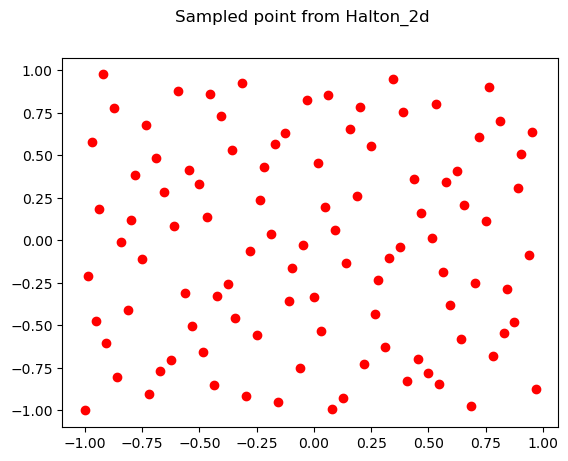
\includegraphics[width=\textwidth]{lab9/imgs/halton.png}
        \caption{Halton sequence}
    \end{subfigure}
    \begin{subfigure}{0.5\textwidth}
        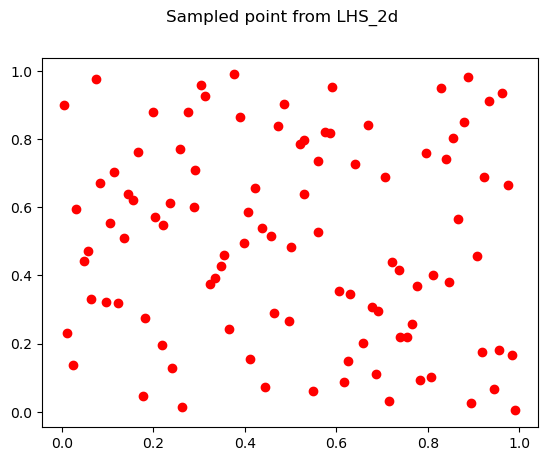
\includegraphics[width=\textwidth]{lab9/imgs/lhs.png}
        \caption{Latin hypercube sampling}
    \end{subfigure}\\
    \begin{subfigure}{0.5\textwidth}
        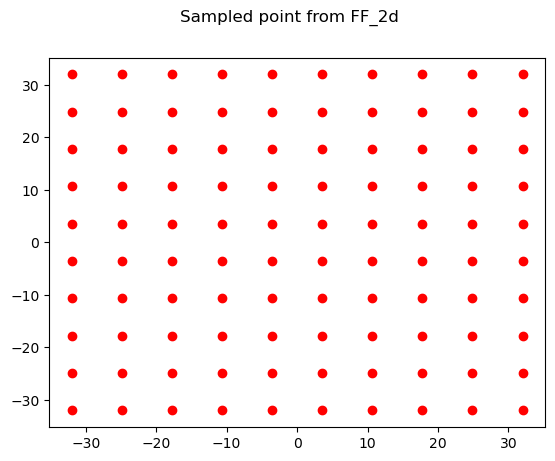
\includegraphics[width=\textwidth]{lab9/imgs/ff.png}
        \caption{Full factorial design}
    \end{subfigure}
    \begin{subfigure}{0.5\textwidth}
        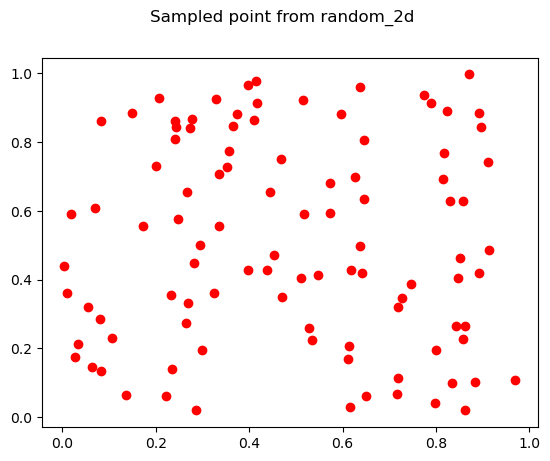
\includegraphics[width=\textwidth]{lab9/imgs/rand.png}
        \caption{Random sampling}
    \end{subfigure}
    \caption{Comparison of different DoE techniques.}
    \label{fig:doe-comp}
\end{figure}

We can see that the methods don't differ much both in terms of total time and in term of mean and standard deviation of the results. The only exception is the full factorial which in some cases finds significantly better results (e.g. DeJong5) while in others (e.g. Rosenbrock, Rastrigin) performs significantly worse. In the Rastrigin function, for example, full factorial works so well because the point it samples is perfectly the global minimum \ref{fig:doe-rastrigin}


\begin{table}[H]
    \centering
    \begin{tabular}{|c|c|c|c|c|c|}
        Function                    & Method         & Mean     & Std. Dev. & Time (s) \\ \hline
        \multirow{4}{*}{Ackley}     & Halton         & 0.7861   & 1.9925    & 14.56    \\
                                    & LHS            & 0.2753   & 0.5453    & 15.38    \\
                                    & Full Factorial & 4.44e-16 & 0.0       & 16.25    \\
                                    & Random         & 0.3867   & 0.88809   & 16.25    \\ \hline
        \multirow{4}{*}{Rastrigin}  & Halton         & 0.4721   & 0.5585    & 17.79    \\
                                    & LHS            & 0.6673   & 0.8143    & 20.66    \\
                                    & Full Factorial & 0.0      & 0.0       & 20.80    \\
                                    & Random         & 0.8337   & 0.9970    & 20.94    \\ \hline
        \multirow{4}{*}{Rosenbrock} & Halton         & 0.0101   & 0.0142    & 17.37    \\
                                    & LHS            & 0.0519   & 0.0747    & 17.83    \\
                                    & Full Factorial & 0.1336   & 0.1468    & 18.61    \\
                                    & Random         & 0.0680   & 0.0948    & 18.48    \\ \hline
        \multirow{4}{*}{DeJong5}    & Halton         & 3.0290   & 2.8565    & 46.83    \\
                                    & LHS            & 4.2475   & 3.3345    & 48.84    \\
                                    & Full Factorial & 0.9980   & 9.41e-05  & 47.08    \\
                                    & Random         & 4.7181   & 3.6863    & 48.31    \\ \hline
    \end{tabular}
    \caption{Results of the comparison of different DoE techniques.}
    \label{tab:doe-comparison}
\end{table}

\begin{figure}[H]
    \centering
    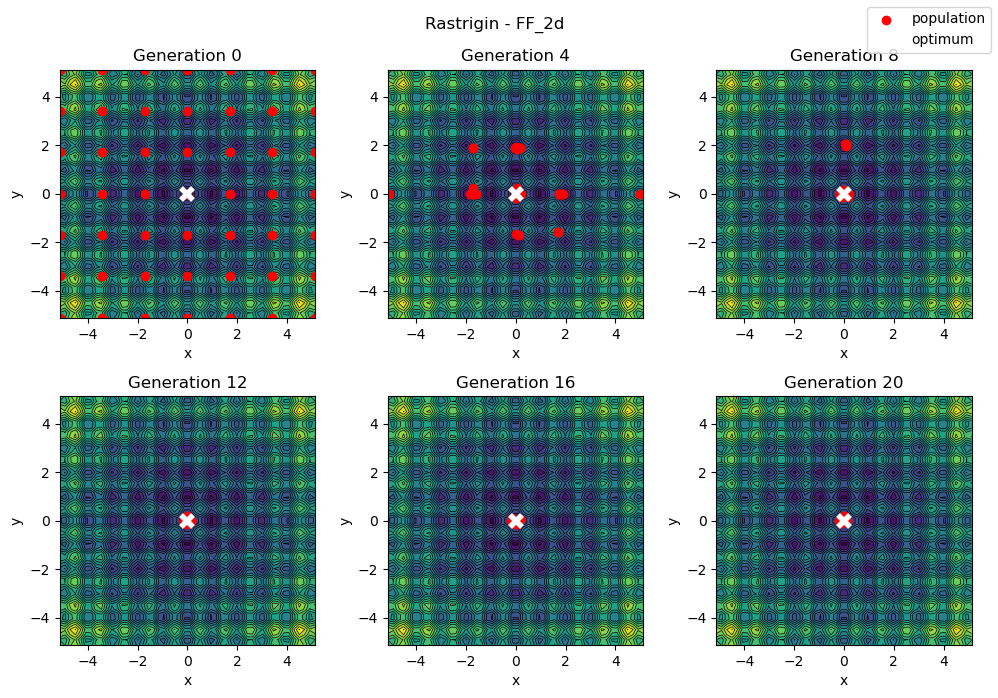
\includegraphics[width=0.8\textwidth]{lab9/imgs/doe_rastrigin.png}
    \caption{Rastrigin function with full factorial design.}
    \label{fig:doe-rastrigin}
\end{figure}